\section{Описание проекта}
\subsection{Авторизация}
Авторизация --- это процесс предоставления определённому лицу или группе лиц прав на выполнение определённых действий. Также сюда входит проверка данных, прав при попытке выполнения этих действий.

\subsection{Аутентификация}
Аутентификация --- процедура проверки подлинности.

\subsubsection{\acrfull{jwt}}
\begin{figure}[h!]
    \begin{center}
        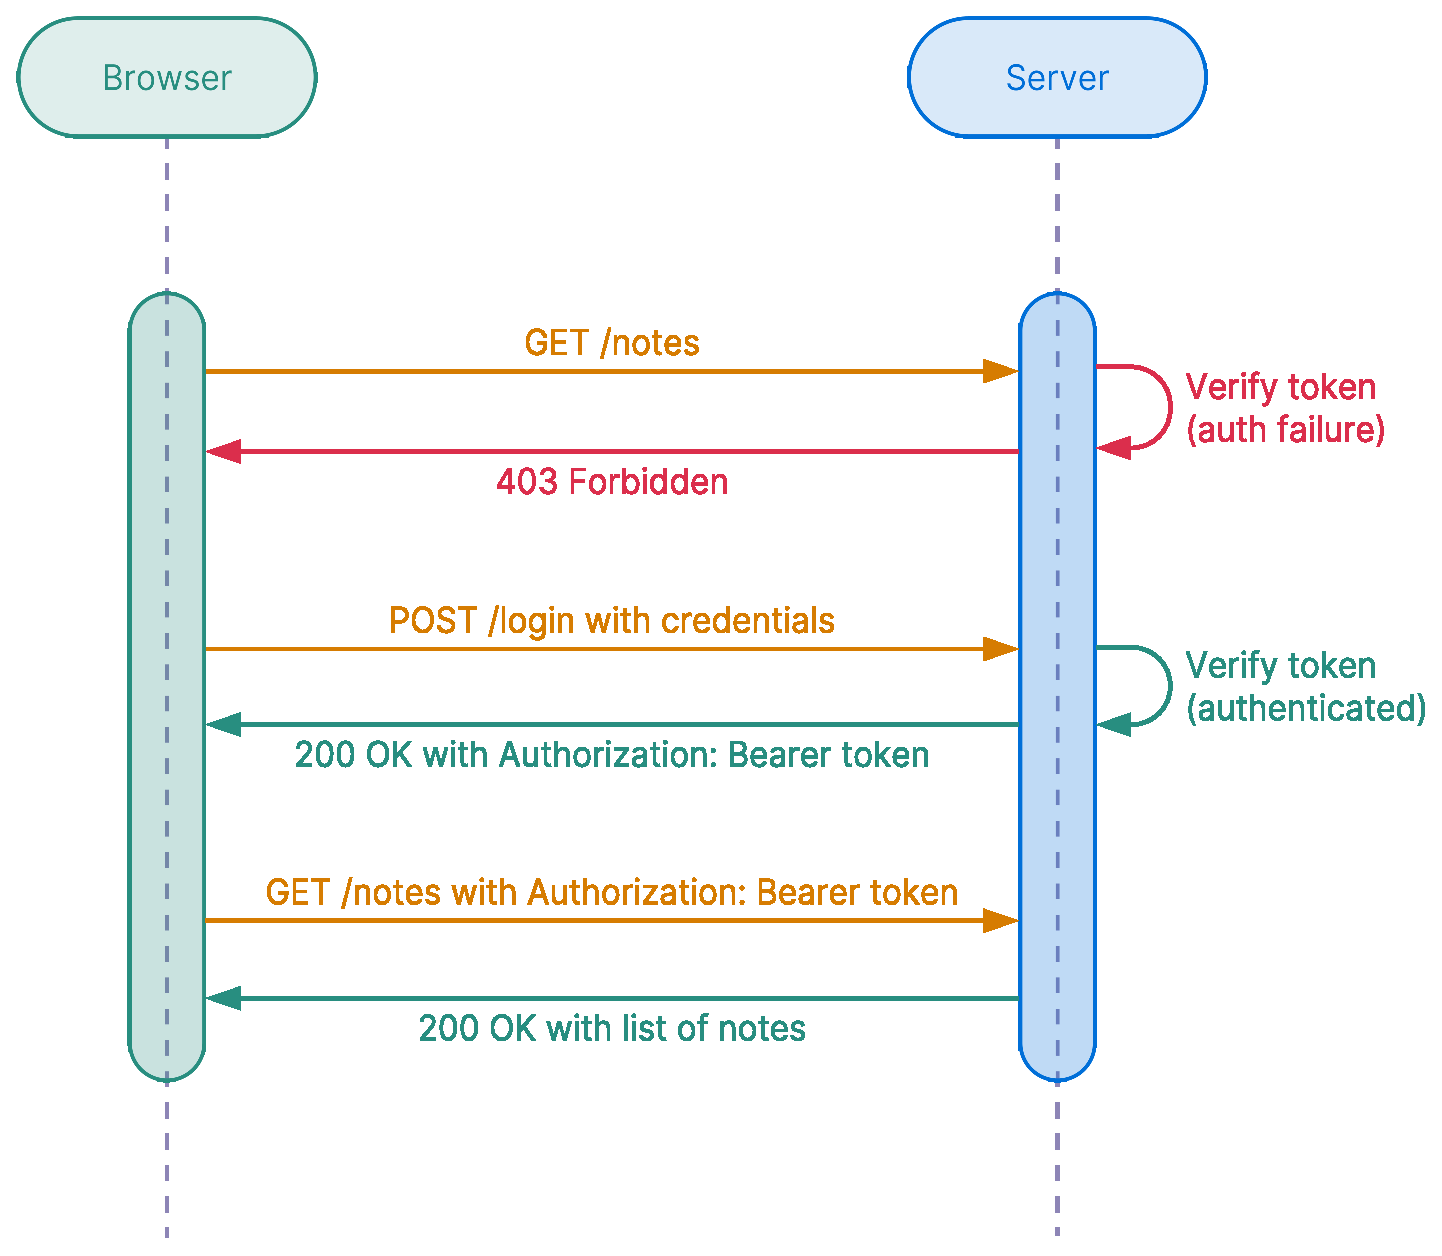
\includegraphics[scale=0.4]{images/jwt-example.eps}
        \caption{Демонстрация работы \acrshort{jwt}}
    \end{center}
\end{figure}

\acrfull{jwt} --- это открытый стандарт \href{https://tools.ietf.org/html/rfc7519}{(RFC 7519)}, который определяет способ для безопасной передачи информации между сторонами с помощью JSON объектов. Эту информацию можно проверить, потому что она имеет цифровую подпись.

\clearpage